\lecture{Finite state methods in NLP}{finstatemeth}

\section{Finite State Automata}

\begin{frame}

	\begin{center}
		\Huge \insertsection
	\end{center}

\end{frame}


\begin{frame}

	\frametitle{\insertsection}
	
	\begin{enumerate}
		\item Finite State Recognizers and Generators
		\begin{enumerate}
			\item Basics and simple machines
			\item Finite State Automata
		\end{enumerate}
		\item Deterministic and Non-deterministic Automata
		\item Implementing FSA in Prolog
		\begin{enumerate}
			\item Defining FSA in Prolog
			\item A Recognizer and Generator in Prolog with no jumps
			\item A Recognizer and Generator in Prolog with jumping arcs
		\end{enumerate}
		\item Finite State Methods in Computational Linguistics and NLP
	\end{enumerate}

\end{frame}

\subsection{Finite State Recognizers and Generators}

\begin{frame}

	\frametitle{\insertsection}
	\framesubtitle{\insertsubsection}
	
	\begin{itemize}
		\item Finite State Automata are used in morphology, phonology, text to speech, and data mining.
		\item They are simple and well understood mathematically.
		\item They are easy to implement and implementations are usually very efficient.
		\item With all simplicity FSA are restricted in what they are able to do.
		\item There is not a finite state solution for every NLP problem.
	\end{itemize}

\end{frame}

\begin{frame}

	\frametitle{\insertsection}
	\framesubtitle{\insertsubsection}
	
	\begin{itemize}
		\item A \textbf{finite state generator} is a simple computing machine that outputs a sequence of symbols.
		\item FSG has a finite number of different states (obviously it has).
		\item It starts in some start state and then tries to reach a final state by making transitions from one state to another. Every time it makes such a transition it \textbf{emits} a symbol.
		\item It cannot stop until it reaches a final state.
		\item FSG only know the state it is currently in, and cannot look ahead at the states that come and also doesn't have any memory of the states it has been.
	\end{itemize}
	
\end{frame}


\begin{frame}

	\frametitle{\insertsection}
	\framesubtitle{\insertsubsection}
	
	\begin{itemize}
		\item Finite state generators can be thought of as directed graphs.
		\item In fact finite state generators are usually drawn as directed graphs.
	\end{itemize}

\end{frame}


\begin{frame}

	\frametitle{\insertsection}
	\framesubtitle{\insertsubsection}

	
	\only<1>{\begin{figure}
		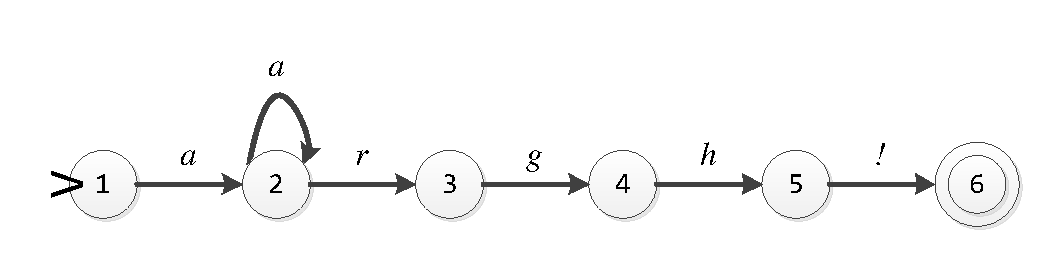
\includegraphics[scale=0.85]{screaming_machine}
	\end{figure}}

	\only<2->{\begin{figure}
			
\includegraphics[scale=0.85]{frustration}
	\end{figure}}
	
\end{frame}


\begin{frame}

	\frametitle{\insertsection}
	\framesubtitle{\insertsubsection}
	
	\begin{itemize}
		\item Finite state recognizers are simple computing machines that read a sequence of symbols from an input tape.
		\item In fact, finite state generators and finite state recognizers are exactly the same kind of machine.
		\item An FSA recognizes (or accepts) a string of symbols \(s_1,s_2,s_3,\ldots \).
		\item Starting in an intial state it can read in the symbols one after the other while making transitions from one state to another such that the transition reading in the last symbol takes the machine into a final state.
		\item An FSA fails to recognize a string if:
		\begin{itemize}
			\item It cannot reach a final state or
			\item it can reach a final state, but when it does there are still unread symbols left over
		\end{itemize}
		
	\end{itemize}

\end{frame}


\begin{frame}

	\frametitle{\insertsection}
	\framesubtitle{\insertsubsection}
	
	
	\begin{figure}
			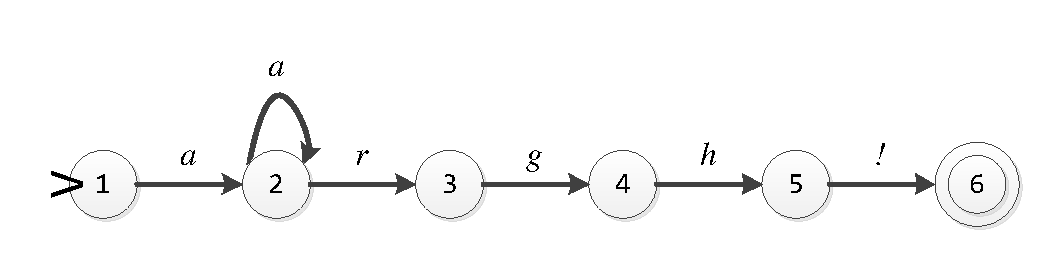
\includegraphics[scale=0.85]{screaming_machine}
	\end{figure}
	

\end{frame}



\begin{frame}

	\frametitle{\insertsection}
	\framesubtitle{\insertsubsection}
	
	
	\begin{itemize}
		\item A formal language is a set of strings.
		\item The language recognized by an FSM is the set of all strings it recognizes when used in recognition mode.
		\item The language generated by an FSM is the set of all strings it can generate when used in generation mode.
		\item The language accepted and the language generated by an FSM are exactly the same.
	\end{itemize}


\end{frame}


\subsection{Some Examples}

\begin{frame}

	\frametitle{\insertsection}
	\framesubtitle{\insertsubsection}
	
	\only<1>{
		Automation with a jump arc.
		\begin{figure}
			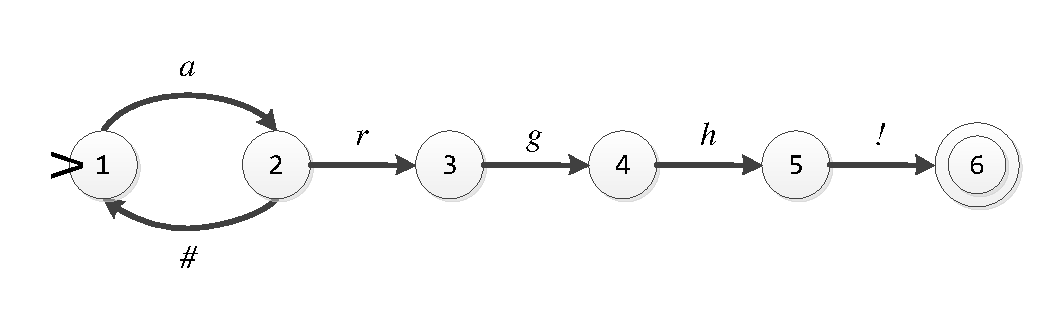
\includegraphics[scale=0.85]{screaming_machine_with_jumps}
		\end{figure}
	}

	\only<2>{
		Another alphabet.
		\begin{figure}
			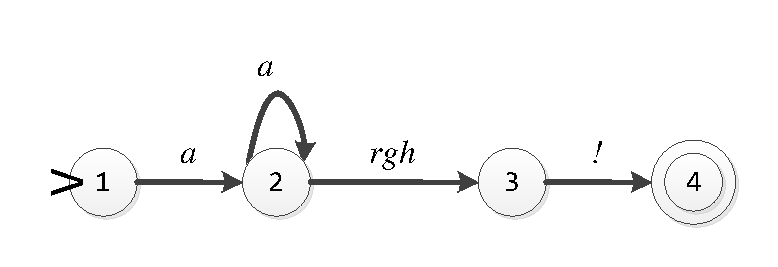
\includegraphics[scale=0.85]{complex_alphabet}
		\end{figure}
	}

	\only<3->{
		Automation with multiple final states.
		\begin{figure}
			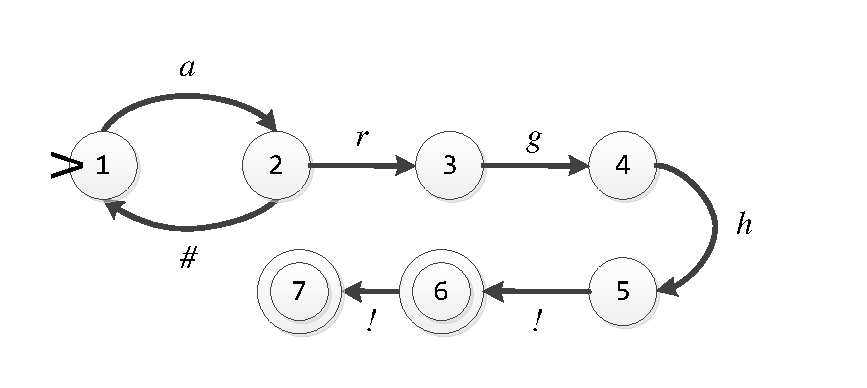
\includegraphics[scale=0.85]{multiple_finals}
		\end{figure}
	}


\end{frame}


\subsection{Deterministic and Non-deterministic Automata}


\begin{frame}

	\frametitle{\insertsection}
	\framesubtitle{\insertsubsection}
	
	
	\begin{figure}
		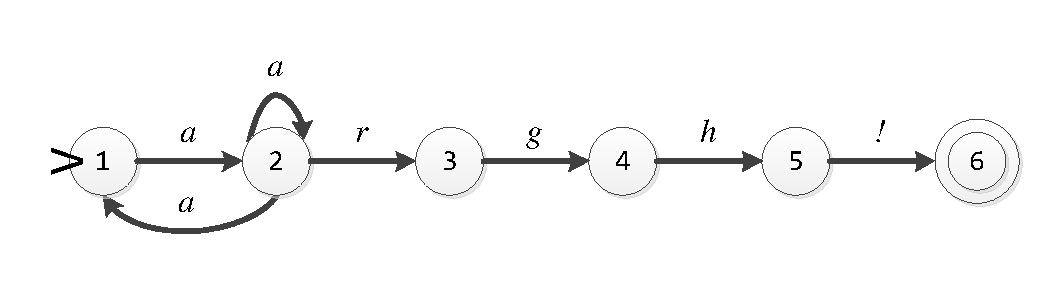
\includegraphics[scale=0.85]{nondet}
	\end{figure}


\end{frame}


\begin{frame}

	\frametitle{\insertsection}
	\framesubtitle{\insertsubsection}
	
	\begin{itemize}
		\item This automation has two arcs labelled with the same symbol going out of one state -- this FSA is \textbf{non-deterministic}.
		\item Non-determinism doesn't add anything to what FSAs can do.
		\item When using an automaton for generation, there is no big difference between deterministic and non-deterministic machines.
		\item There is, however, a difference when we want to use the machine for recognition: non-determinism brings with it the need to perform \textbf{search}.
	\end{itemize}

\end{frame}


\subsection{Implementing FSA in Prolog}


\begin{frame}

	\frametitle{\insertsection}
	\framesubtitle{\insertsubsection}
	
	\begin{itemize}
		\item We are going to treat FSAs as passive data structures that are manipulated by other programs.
		\item Separating declarative and procedural information is often a good idea.
		\item We will use three predicates to represent FSAs:
		\texttt{\begin{enumerate}
			\item start/1
			\item end/1
			\item arc/3
		\end{enumerate}}
	\end{itemize}

\end{frame}


\begin{frame}

	\frametitle{\insertsection}
	\framesubtitle{\insertsubsection}
	
	\only<1>{
		Simple screaming machine
		\texttt{\begin{itemize}
			\item[] start(1).
			\item[] end(6).
			\item[] arc(1,2,a).
			\item[] arc(2,3,r).
			\item[] arc(2,2,a).
			\item[] arc(3,4,g).
			\item[] arc(4,5,h).
			\item[] arc(5,6,!).
	\end{itemize}}}

	\only<2>{
		Non-deterministic screaming machine
		\texttt{\begin{itemize}
				\item[] start(1).
				\item[] end(6).
				\item[] arc(1,2,a).
				\item[] arc(2,3,r).
				\item[] arc(2,1,a).
				\item[] arc(2,2,a).
				\item[] arc(3,4,g).
				\item[] arc(4,5,h).
				\item[] arc(5,6,!).
	\end{itemize}}}

	\only<3->{
		Screaming machine with a jumping arc
		\texttt{\begin{itemize}
				\item[] start(1).
				\item[] end(6).
				\item[] arc(1,2,a).
				\item[] arc(2,3,r).
				\item[] arc(2,1,'\#').
				\item[] arc(3,4,g).
				\item[] arc(4,5,h).
				\item[] arc(5,6,!).
	\end{itemize}}}

\end{frame}


\begin{frame}

	\frametitle{\insertsection}
	\framesubtitle{\insertsubsection}
	
	\only<1>{
		\textbf{Recognizer and Generator without jump arcs}
		\texttt{\begin{itemize}
				\item[] recognize(Node,[]) :- end(Node).
				\item[] recognize(Node,String) :- arc(Node,Next,Label), \\ \quad\quad\quad\quad\quad\quad\quad\quad\quad\quad\quad\quad traverse(Label,String,NewStr), \\ \quad\quad\quad\quad\quad\quad\quad\quad\quad\quad\quad\quad recognize(Next,NewStr).
				\item[] traverse(Label,[Label|Symbols],Symbols).
				\item[] run(Symbols) :- start(Node),recognize(Node,Symbols).
	\end{itemize}}}

	\only<2->{
		\textbf{Recognizer and Generator with jump arcs}
		\texttt{\begin{itemize}
				\item[] recognize1(Node,[]) :- end(Node).
				\item[] recognize1(Node,String) :- arc(Node,Next,Label), \\ \quad\quad\quad\quad\quad\quad\quad\quad\quad\quad\quad\quad
				traverse1(Label,String,NewStr), \\ \quad\quad\quad\quad\quad\quad\quad\quad\quad\quad\quad\quad
				recognize1(Next,NewStr).
				\item[] traverse1('\#',String,String).
				\item[] traverse1(Label,[Label|Symbols],Symbols).
				\item[] run1(Symbols) :- start(Node),recognize1(Node,Symbols).
	\end{itemize}}}

\end{frame}


\subsection{Finite State Methods in Computational Linguistics and NLP}


\begin{frame}

	\frametitle{\insertsection}
	\framesubtitle{\insertsubsection}
	
	\begin{itemize}
		\item Finite state machines are very simple, but there are limitations to what they can do.
		\item FSA can only recognize and generate \textbf{Regular Languages}.
		\item Many linguistic phenomena can only be described by languages which cannot be generated by FSAs.
		\item There are, however, linguistic applications where the expressive power of finite state methods seems to be sufficient.
		\item Finite state methods have been shown to be particularly useful are phonological and morphological processing, and have also been applied to syntactic analysis.
	\end{itemize}

\end{frame}